% Chapter 1 (from pres-main tex file)
% New Trends in Research
% Author: Javier Reyes

\subsection{Vivado HLx}

\begin{frame}
	\frametitle{Vivado HLx}
	Replacing ISE tools, the tool suite allows design, integration and implementation of systems for the Xilinx technologies.
	\vfill
	Included programs:
	\begin{itemize}
		\item Vivado HLx - High Level design
		\item Xilinx SDK - Software development 
		\item Vivado HLS - High Level Synthesis
		\item (Optional, external) Petalinux - Embedded Linux image building
	\end{itemize}
\end{frame}

\begin{frame}
	\frametitle{Vivado HLx}
	\begin{itemize}
		\item Interaction through GUI or native embedded TCL scripting language (commands either through the IDE console, or as file scripts). 
		\item Runs under Windows and Linux\footnote[frame]{Distro dependant, see \cite{UG973}} OS.
	\end{itemize}
\end{frame}

\begin{frame}
	\frametitle{IDiAL Server}
	Given the high requirements and the need to mantain a common work platform, a Virtual Machine is created in the IDiAL Server, where the tools are available to create/modify the designs.
	\vfill
	\begin{itemize}
		\item VM: U16x64D\_Vivado
		\item User: Javier
		\item Password: IDiAL
		\item OS: Ubuntu 16.04.3 Desktop
		\item IP-Address: 172.22.167.120
	\end{itemize}
\end{frame}

\begin{frame}[fragile]
	\frametitle{Basic install \& launch}
	\begin{lstlisting}[language=bash, basicstyle=\tiny\ttfamily, tabsize=2, commentstyle=\color{darkgray}, keywordstyle=\color{blue}, backgroundcolor=\color{lightgray}, morekeywords={chmod, sudo}, breaklines=true]
# Give executable permission to the installer file
chmod +x <installer_filename>.bin
# Executes the installer with root privileges
# Select the WebPack edition - no cost
# Include at least the SDK and the device Zynq in the content selection
# Select the installation folder
sudo ./<installer_filename>.bin
# After install, change to the driver cable installer folder
cd <vivado_folder>/data/xicom/cable_drivers/lin64/install_script/install_drivers/
# Execute the driver cable installer with root privileges
sudo ./install_drivers
# Create the apropiate environment for the suite to be launched
# Needs to be run everytime before launching Vivado
# Alternatively, can be added to the .bashrc to be executed automatically
source _vivado_installed_folder_/settings64.sh
# Launch the Vivado GUI, blocks the terminal when launched
vivado &
	\end{lstlisting}
	\begin{alertblock}{Constraint}
		{\small The Windows installer runs automatically the USB drivers, while in Linux it needs to be run after the Installation.}
	\end{alertblock}
\end{frame}

\begin{frame}
	\frametitle{Hardware Project}
	\begin{columns}
		\begin{column}{0.5\textwidth}
			\begin{figure}
				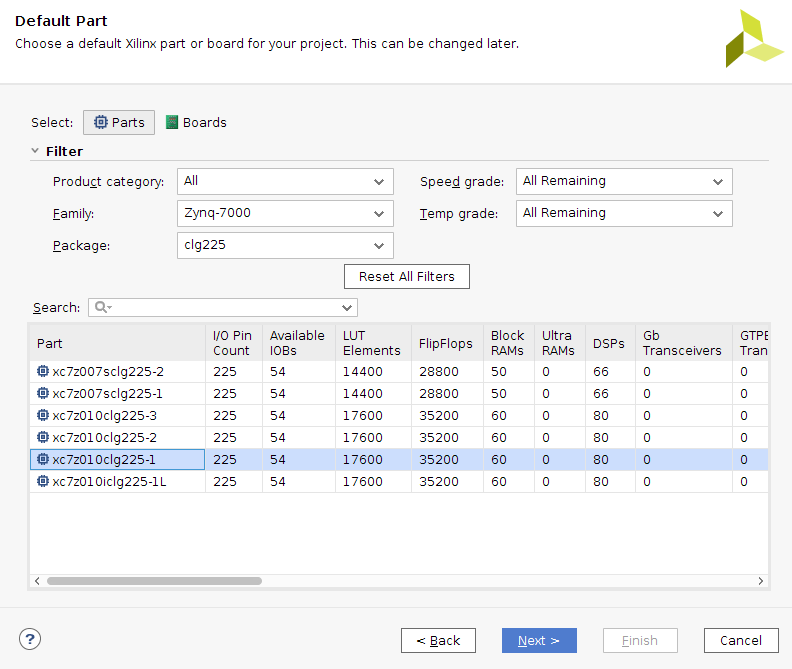
\includegraphics[width=\textwidth]{project-device.png}
				\caption{Vivado project - Device selection.}\label{fig:project-device}
			\end{figure}
		\end{column}
		\begin{column}{0.5\textwidth}
			\begin{itemize}
				\item Create a new project.
				\item Select RTL project type.
				\item Select the correspondent device.
				\item Create a new Block Design.
				\item Add the Zynq7 IP Core.
				\item Add/create any other necesary IP Core.
				\item Configure the IP Core.
			\end{itemize}
		\end{column}
	\end{columns}
\end{frame}

\begin{frame}
	\frametitle{Hardware Project}
	\begin{columns}
		\begin{column}{0.5\textwidth}
			\begin{figure}
				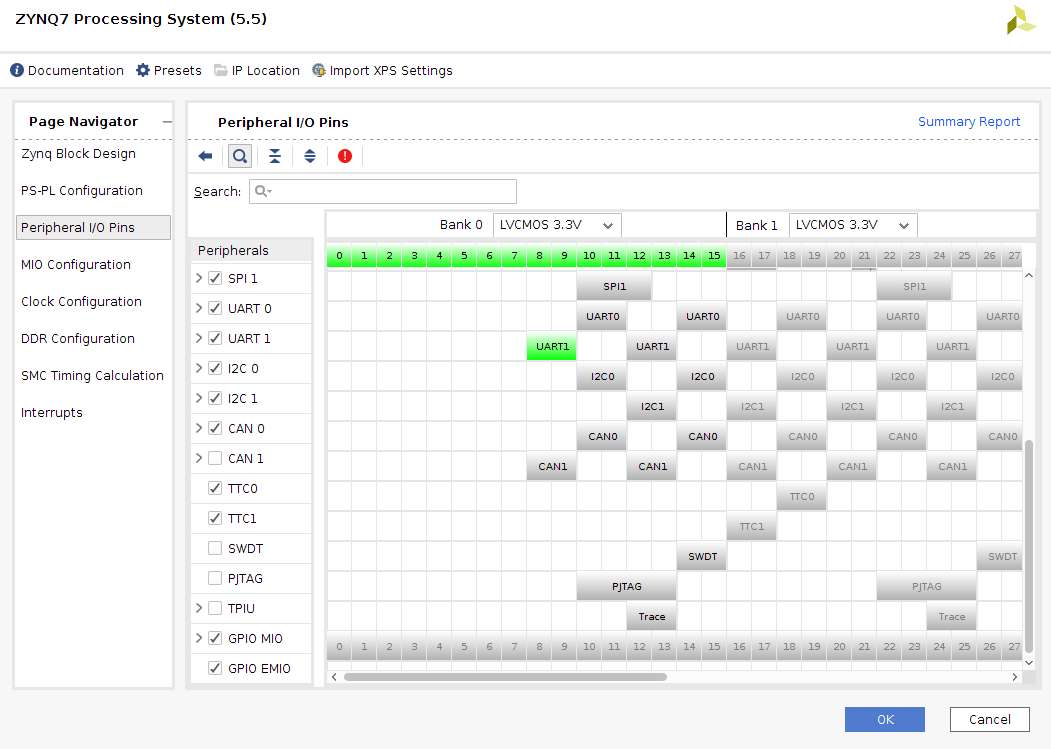
\includegraphics[width=\textwidth]{can-enable.png}
				\caption{Vivado project - IP Core configuration.}\label{fig:can-enable}
			\end{figure}
		\end{column}
		\begin{column}{0.5\textwidth}
			\begin{itemize}
				\item Apply the configuration in the TCL script, provided by the manufacturer.
				\item Enable all the required peripherals (CAN, USB, etc).
				\item Route all the enabled modules to an available MIO pin or via EMIO.
				\item Configure the frequency for the CAN REF CLK signal (80 MHz).
			\end{itemize}
		\end{column}
	\end{columns}
\end{frame}

\begin{frame}
	\frametitle{Hardware Project}
	\begin{columns}
		\begin{column}{0.5\textwidth}
			\begin{figure}
				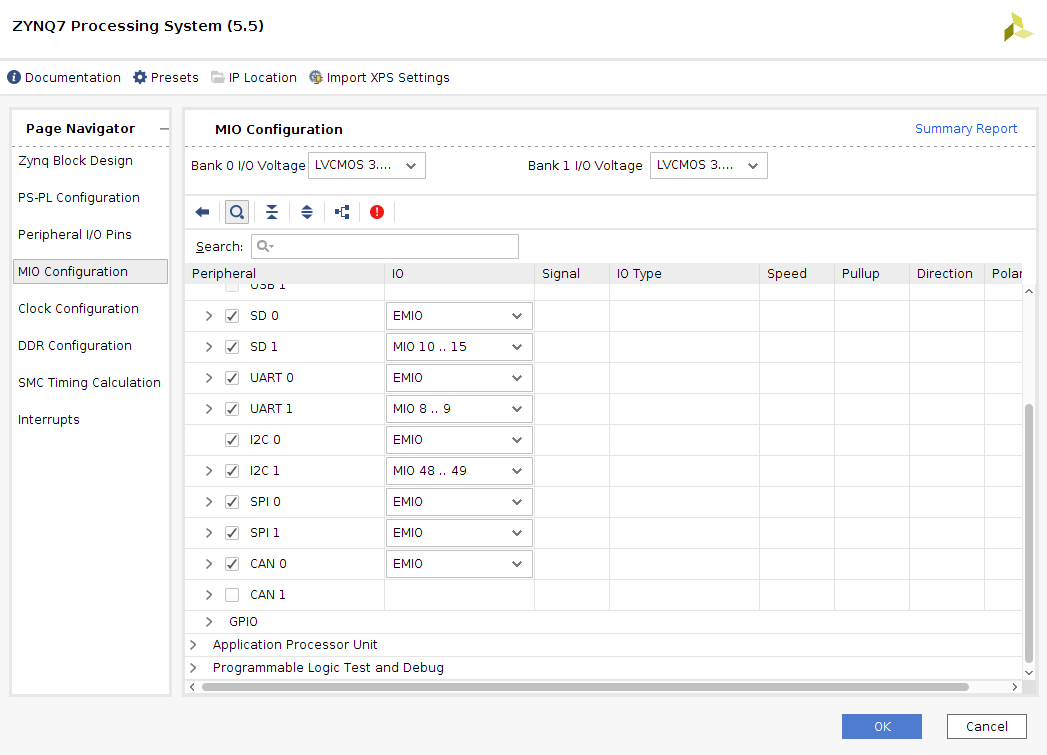
\includegraphics[width=\textwidth]{can-emio.png}
				\caption{Vivado project - Signals routing.}\label{fig:can-emio}
			\end{figure}
		\end{column}
		\begin{column}{0.5\textwidth}
			\begin{figure}
				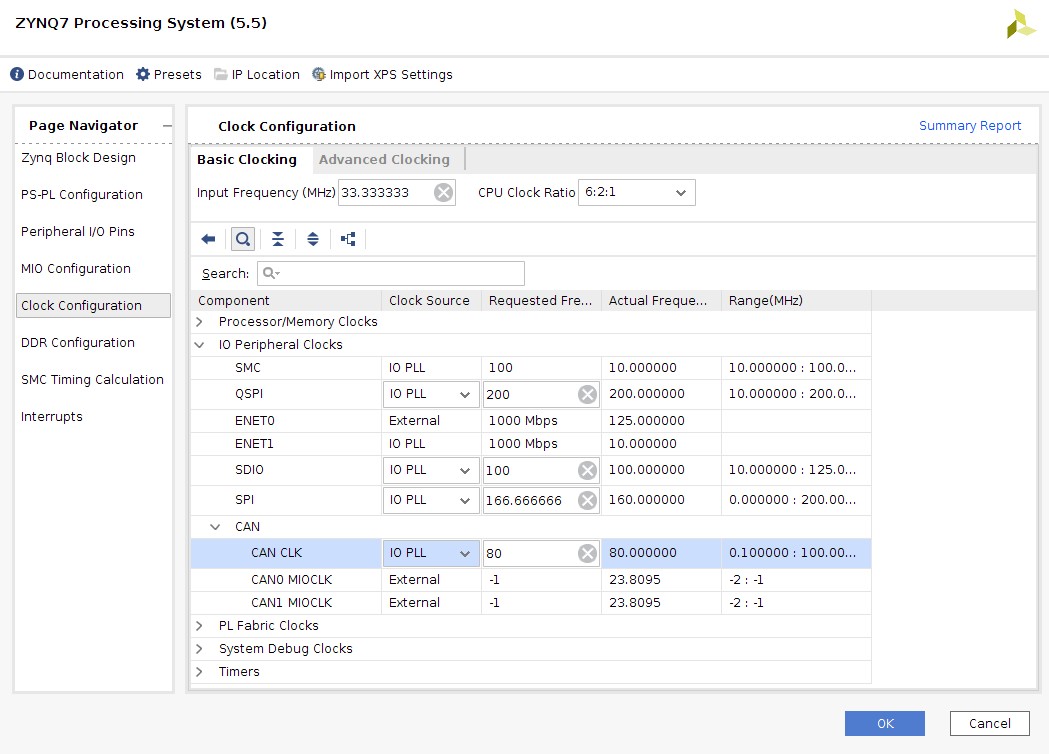
\includegraphics[width=\textwidth]{can-clock.png}
				\caption{Vivado project - Clock configuration.}\label{fig:can-clock}
			\end{figure}
		\end{column}
	\end{columns}
\end{frame}

\begin{frame}
	\frametitle{Hardware Project}
	\begin{columns}
		\begin{column}{0.5\textwidth}
			\begin{figure}
				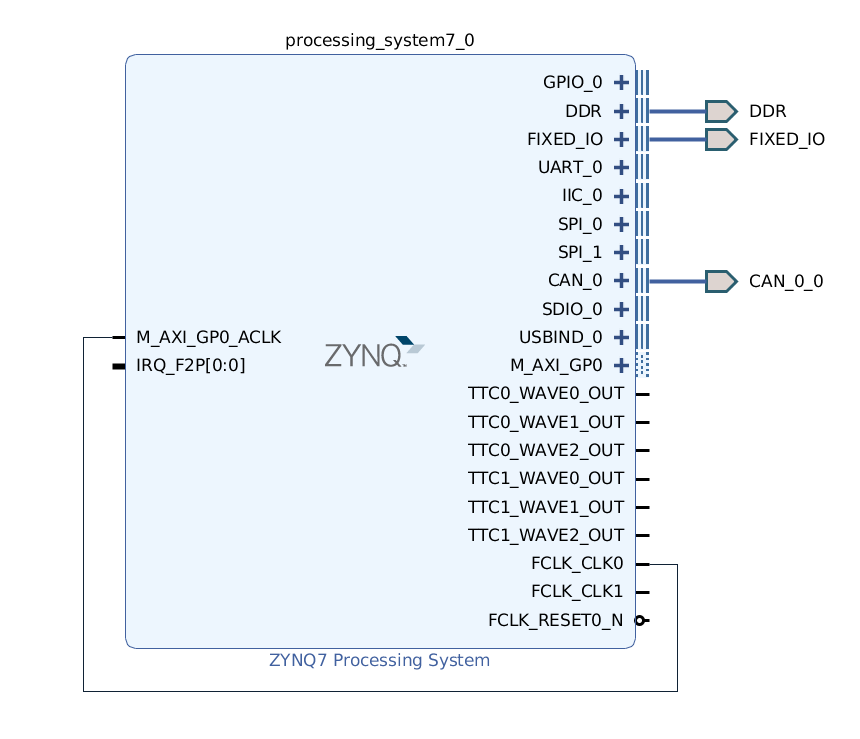
\includegraphics[width=\textwidth]{ip-core.png}
				\caption{Vivado project - Block Design.}\label{fig:ip-core}
			\end{figure}
		\end{column}
		\begin{column}{0.5\textwidth}
			\begin{itemize}
				\item Run the Block Automation wizard.
				\item Run the Connection Automation wizard.
				\item Set all signals that will be routed to a physical pin external (Make external).
				\item Generate an HDL wrapper for the Block Design.
				\item Open the Elaborated Design (RTL Analysis), and set the I/O planning layout.
			\end{itemize}
		\end{column}
	\end{columns}
\end{frame}

\begin{frame}
	\frametitle{Hardware Project}
	\begin{columns}
		\begin{column}{0.5\textwidth}
			\begin{figure}
				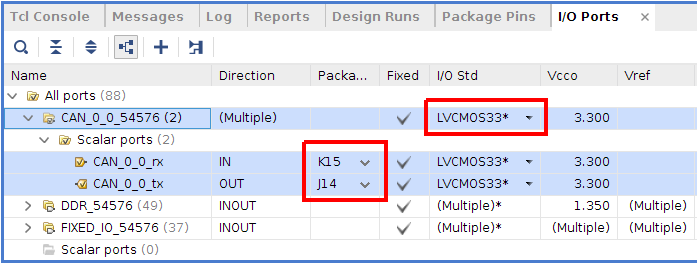
\includegraphics[width=\textwidth]{set-constraints.png}
				\caption{Vivado project - External pins mapping.}\label{fig:set-constraints}
			\end{figure}
		\end{column}
		\begin{column}{0.5\textwidth}
			\begin{itemize}
				\item Config the IO standard and package pin for the external signals (see Trenz TRM \cite{zynq-trm}).
				\item Run Synthesis, Implementation and Generate Bitstream.
				\item Export hardware, including bitstream file.
				\item Launch SDK, selecting the local project environment.
			\end{itemize}
		\end{column}
	\end{columns}
\end{frame}

\begin{frame}
	\frametitle{Hardware Project}
	\begin{columns}
		\begin{column}{0.5\textwidth}
			\begin{figure}
				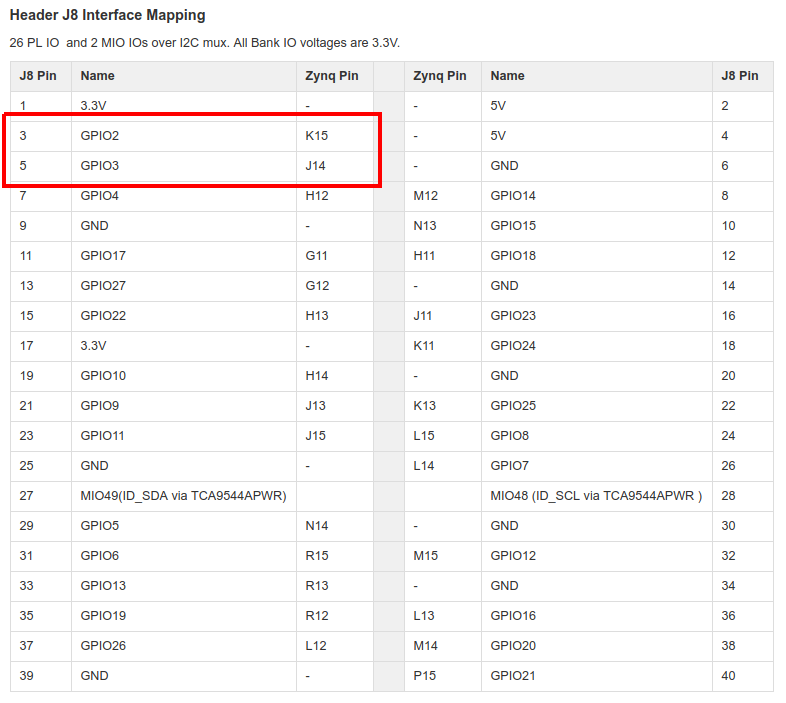
\includegraphics[width=\textwidth]{zynq-pins.png}
				\caption{Vivado project - Mapped pins location.}\label{fig:zynq-pins}
			\end{figure}
		\end{column}
		\begin{column}{0.5\textwidth}
			\begin{figure}
				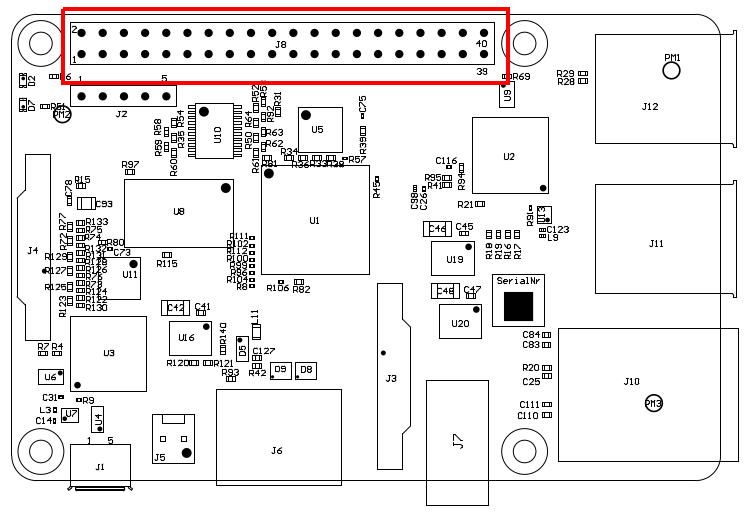
\includegraphics[width=\textwidth]{header-pins.png}
				\caption{Vivado project - Header pins identification.}\label{fig:header-pins}
			\end{figure}
		\end{column}
	\end{columns}
\end{frame}

\begin{frame}[fragile]
	\frametitle{GUI Vs. TCL Console}
	Vivado includes a TCL scripting language integrated, for more complex designs. The entire GUI interaction can be translated into TCL command.
	\lstinputlisting[language=tcl, basicstyle=\tiny\ttfamily, tabsize=2, commentstyle=\color{darkgray}, keywordstyle=\color{blue}, backgroundcolor=\color{lightgray}, morekeywords={create_project, create_bd_design, update_compile_order, create_bd_cell, apply_bd_automation}, firstline=1, lastline=10, breaklines=true, numbers=left]{../../../git/DAEbot/Devices/Zynqberry_OperatorPlus/zynqberryHW_CAN/create_project.tcl}
\end{frame}

\subsection{Xilinx SDK}

\begin{frame}
	\frametitle{Software Project}
	Based on the Eclipse SDK, for application development on Zynq Ultrascale+ MPSoC and Zynq-7000 All Programmable families.
	\vfill
	\begin{columns}
		\begin{column}{0.5\textwidth}
			\begin{itemize}
				\item Editor
				\item Compilers
				\item Build tools
				\item Flash memory Management
				\item JTAG debug integration
			\end{itemize}
		\end{column}
		\begin{column}{0.5\textwidth}
			\begin{itemize}
				\item Hierarchical Profiling
				\item Bare-Metal and Linux development
				\item Homogeneous and heterogeneous multi-processor support
			\end{itemize}
		\end{column}
	\end{columns}
\end{frame}

\begin{frame}
	\frametitle{Software Project structure}
	\begin{columns}
		\begin{column}{0.5\textwidth}
			\begin{figure}
				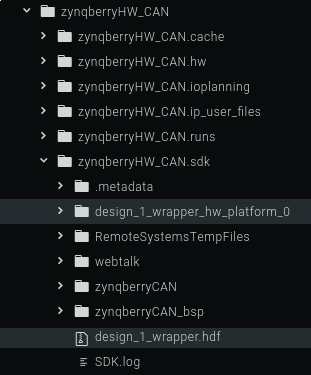
\includegraphics[width=0.8\textwidth]{xilinx-project-structure.png}
				\caption{Xilinx project structure.}\label{fig:xilinx-project-structure}
			\end{figure}
		\end{column}
		\begin{column}{0.5\textwidth}
			\begin{block}{Design aware}
				The software project is handled inside the Vivado project environment, and asimilates the Hardware design to configure Software parameters.
			\end{block}
		\end{column}
	\end{columns}
\end{frame}

\begin{frame}
	\frametitle{Integration issue}
	When the hardware project is exported and SDK is launched with the workspace local to the hardware project, The SDK folder gets linked to the hardware platform designed.
	\vfill
	\begin{alertblock}{Duplicate files/folers alert}
		If a change is made in the hardware project \textbf{after} the SDK project is created, Vivado will create a second hardware platform into SDK. Care need to be taken regardless hardware version, and duplicate files.
	\end{alertblock}
\end{frame}

\begin{frame}[fragile]
	\frametitle{Board Support Package}
	\begin{columns}
		\begin{column}{0.5\textwidth}
			Once the Hardware Platform is imported into SDK, a \textbf{Board Support Package} (BSP) needs to be created. \\
			\vspace{1em}
			It can be created either independent, or as part of a Software Application Project.
		\end{column}
		\begin{column}{0.5\textwidth}
			SDK includes the following BSP:
			\begin{itemize}
				\item Standalone - single-threaded environment, basic features (std IO, hardware access).
				\item Xilkernel - lightweight kernel with POSIX style services (scheduling, threads, synchronization, etc.).
			\end{itemize}
		\end{column}
	\end{columns}
\end{frame}

\begin{frame}
	\frametitle{Board Support Package}
	\begin{columns}
		\begin{column}{0.5\textwidth}
			The BSP provides drivers and libraries (lower layer software stack) for the specific hardware designed.
		\end{column}
		\begin{column}{0.5\textwidth}
			When built, BSP include automatically:
			\begin{itemize}
				\item Standard C libraries
				\item Device Drivers for all peripherals
			\end{itemize}
		\end{column}
	\end{columns}
\end{frame}

\begin{frame}
	\frametitle{BSP Reconfiguration}
	The BSP can be configured and recompiled, to include additional libraries, or setup the parameters for the available drivers.
	\vfill
	\begin{alertblock}{Update needed}
		As the standalone applications may need a console to interact with, the STDIN and STDOUT are linked by default to UART0. In the Zynberry 726, the USB-serial converter is connected to the UART1. In order to use a console terminal, this needs to be changed.
	\end{alertblock}
\end{frame}

\begin{frame}
	\frametitle{SDK Project structure}
	\begin{columns}
		\begin{column}{0.25\textwidth}
			\begin{figure}
				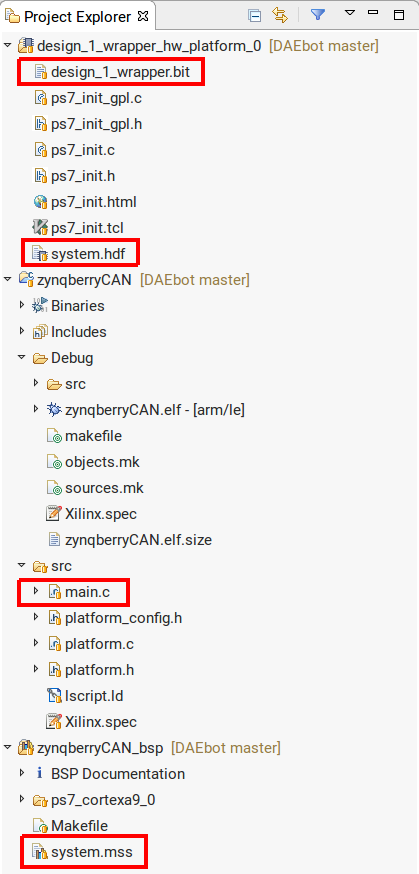
\includegraphics[width=\textwidth]{sdk-projects.png}
				\caption{SDK project structure.}\label{fig:sdk-projects}
			\end{figure}
		\end{column}
		\begin{column}{0.6\textwidth}
			\begin{alertblock}{Files duplication}
				The file linking/management in Xilinx and SDK tools uses copy commands for file management. It can lead to duplicated files. Relevant if the file is modified post-creation.
			\end{alertblock}
		\end{column}
	\end{columns}
\end{frame}

\begin{frame}
	\frametitle{CAN module driver - BSP}
	The BSP provides the driver module for CAN. An example snippet:
	\vfill
	\lstinputlisting[language=C, basicstyle=\tiny\ttfamily, tabsize=2, commentstyle=\color{darkgray}, keywordstyle=\color{blue}, backgroundcolor=\color{lightgray}, morekeywords={s32, u8, u32, XCanPs, NULL}, firstline=908, lastline=924, breaklines=true, numbers=left]{../../../git/DAEbot/Devices/Zynqberry_OperatorPlus/zynqberryHW_CAN/zynqberryHW_CAN.sdk/zynqberryCAN/src/main.c}
\end{frame}
